\chapter{Introduction}
(Start with a motivating scenario: either Powerpoint presentation or USAR
application.)
% \begin{quotation}
% \textit{Imagine an earthquake has hit a populous area and many major roads are
% impassable. Buildings are severely damaged or collapsed, and fire has broken out
% in many places. At the crisis management center, response professionals are
% working together to coordinate the earthquake relief effort. You are the
% incident commander charged with coordinating the search
% and rescue teams working in the field. There is a large tabletop display in
% front of you, showing the map of the site. Information coming from the field is
% updated on the display in real-time.}
% 
% \textit{A report about a big explosion at a chemical plant comes in and you move
% the map around, zoom in and rotate it to get a good view of the plant. On the
% map, you see there is a group of unmanned vehicles nearby. After selecting them
% on the map with your hand, you speak to the interface ``Go nearer to the
% explosion site to gather more information,'' while tracing the route the
% vehicles should take to avoid obstacles. Then you instruct rescue team No. 3 to evacuate the residents
% in the surrounding buildings by going under a bridge because the surface of the
% bridge is blocked. You gesture with one hand as the bridge and the other
% hand moving under it to emphasize this.}
% \end{quotation}
% 
% The scenario above is an example in the Urban Search and Rescue (USAR) domain.
% It shows an application of a multi-modal interface to a real-world problem. Gestures play an important part in this scenario,
% providing key information about location, method and timing of movements,
% and about spatial relationship among the objects being described.

Recent trends in user interfaces have brought on a new wave of interaction
techniques that depart from the traditional mouse and keyboard that have been 
used for decades. These include multi-touch interfaces such as the 
iPhone, the iPad and the Microsoft 
Surface\textsuperscript{\textregistered} as well as camera-based systems such as
the Microsoft Kinect and the Nintendo\textsuperscript{\textregistered} Wii. Most
of these devices gained instant popularity among consumers, and the common trait
among them is that they make interacting with computation more natural and 
effortless. All these devices allow users to use their hands and/or body 
gestures to directly manipulate the virtual objects. It feels more natural this 
way because this is how we interact with our environment in everyday life.
 
(Mention recent trend in wearable computing: Google Glass, Samsung Galaxy Gear
and Pebble.) 

Our goal is to take this aspiration to the next level by developing
an intelligent multi-modal interface for natural interaction. By \textit{natural
interaction}, we mean the kind of cognitively transparent, effortless
multi-modal communication that can happen between people; we want to make this possible in
human-computer interaction such that the computer interface understands what the
user is saying and doing, and the user can simply behave. We believe that
natural interaction can provide better learnability, flexibility, memorability,
convenience and efficiency, but further user studies are needed to investigate
this belief.

Gesture plays an important part in multi-modal interaction, especially for
conveying spatial information. The focus of this thesis is developing a
hierarchical approach for continuous gesture analysis that can be easily
applied in different domains and applications. Specifically, we focus on
gestures made with hands. 

I propose a gesture-based interface that allows users to perform
manipulative (continuous) and communicative (discrete) gestures continuously
with no arbitrary restrictions. The key elements of the approach are the hierarchical framework
for gestural analysis based on abstract hidden Markov models (AHMMs) and the
accurate real-time detection of the onset of natural gestures that convey 
information intended by the users, while filtering out movements that do not 
convey information.

\section{Background}
\subsection{Definition of Gestures}
Webster's Dictionary defines gestures as ``\ldots the use of motions of the
limbs or body as a mean of expression; a movement usually of the body or limbs
that expresses or emphasizes an idea, sentiment, or attitude.'' This definition
is particularly related to the communicational aspect of the human hand and body
movements. However, in the domain of human computer interaction (HCI) the notion
of gestures is somewhat different. In their review of the visual interpretation
of hand gestures for HCI, Pavlovic et al. \cite{Pavlovic97} states that in a computer
controlled environment one wants to use the human hand to perform tasks that
mimic both the natural use of the hand as a manipulator, and its use in
human-machine communication. They include both manipulative and communicative
gestures in their gesture taxonomy. This is also the definition we will use in
this thesis.

Pavlovic et al. \cite{Pavlovic97} also gives a model (Figure. 
\ref{fig:gesture_production}) for the production and perception of gestures 
based on the model used in the field of spoken language recognition. According 
to their model, gestures originate as a gesturer's mental concept, possibly in 
conjunction with speech. They are expressed through the motion of arms and 
hands. Also, observers perceive gestures as streams of visual images which they
interpret using their knowledge about those gestures. In HCI, the 
observer is the computer and the knowledge it possesses is the training data we 
give it.

\begin{figure}[h]
  \centering
  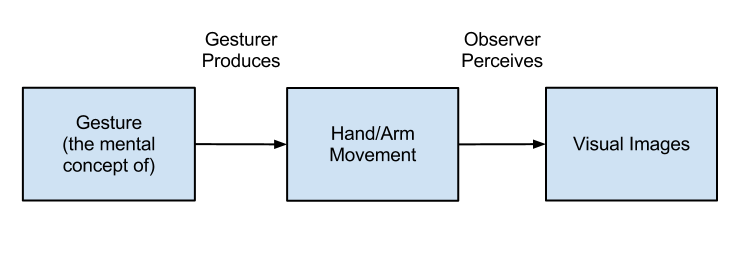
\includegraphics[width=0.7\textwidth]{figures/gesture_production.png} 
  \caption{Production and perception of gestures. Hand gestures originate as a
  mental concept, are expressed through arm and hand motion, and are perceived
  as visual images \cite{Pavlovic97}.}
  \label{fig:gesture_production}
\end{figure}

\subsection{Gestural Taxonomy}\label{sec:taxonomy}
The mental concept of a gesture represents the semantic meaning or the
actual intention of the gesturer. In this dimension, hand movements can be
divided into different general categories. Each category has its own characteristics and requires different responses from the computer interface. Having a systematic gesture taxonomy can inform
us about the design of the interactive system. The taxonomy will also be the
basis of our hierarchical approach to gesture interpretation. Our gesture
taxonomy (see Figure \ref{fig:taxonomy}) is based on the one developed by Pavlovic et al.
\cite{Pavlovic97} with some changes to make the terminology clearer. This is
also similar to the \textit{nature} dimension in the taxonomy proposed by
Wobbrock et al. \cite{wobbrock09}

\begin{figure}[h]
  \centering
  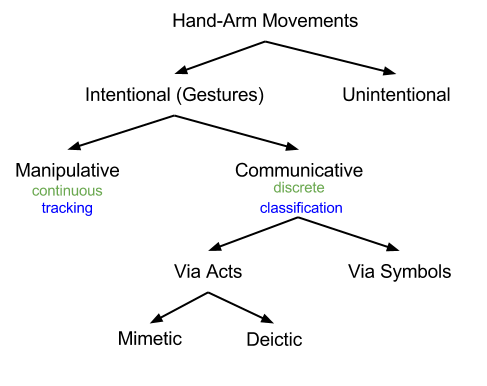
\includegraphics[width=0.5\textwidth]{figures/taxonomy.png} 
  \caption{Gesture taxonomy}
  \label{fig:taxonomy}
\end{figure}

First, gestures, as \textit{intentional} movements, should be distinguished from
\textit{unintentional} hand movements (like beats). By \textit{unintentional}
movements, we mean movements that are not intended to convey information. In
contrast, gestures are meaningful hand movements that people make to convey some
information. The distinction is important for a natural interface because there
should not be any restriction on how people should place or move their hands
when they are not doing any meaningful gestures. 

Gestures are then further divided into manipulative and communicative
categories. Manipulative gestures are used to act on objects (e.g.
moving an virtual object around, click a button, the property of the virtual
object change directly according to certain parameters of the hand(s)), while
communicative gestures have an inherent purpose for communication \cite{Pavlovic97}. 
the meaning of the gesture when the user finishes performing the gesture. This part is
accomplished by gesture recognition. So manipulative gestures and communicative
gestures fall into the \textit{continuous} category and the
\textit{discrete} category respectively in the \textit{flow} dimension of the
taxonomy proposed by Wobbrock \cite{wobbrock09} et al. based on their
user study.

People perform communicative gestures via acts or symbols. Gesture via acts are
those directly related to the interpretation of the movement itself. Such
movements are classified as either mimetic (which imitate some actions) or
deictic (pointing acts that convey spatial information). Gestures via symbols
are those that have a linguistic role, and are often represented by different static hand postures. An example is forming the
O.K. pose for ``accept''. 

The physical arm and hand movements that express the mental concept of the
gesture can be categorized into different \textit{forms} \cite{wobbrock09} as
shown in Table \ref{tab:form}. Both manipulative and communicative gestures can
have all of these forms. This means that the features we want to use for
gestural analysis should be based on both the hand pose and the locus of the
hand movement.

\begin{table}[h]
  \centering
  \begin{tabular}{| l | l |}
  	\hline
  	\textbf{Form} 		  & \textbf{Description} \\ \hline 
  	Static pose  		  & Hand pose is held in one location. \\ \hline
  	Dynamic pose 		  & Hand pose changes while location does not. \\ \hline
  	Static pose and path  & Hand pose is held as hand moves. \\ \hline
  	Dynamic pose and path & Hand pose changes as hand moves. \\ \hline
  \end{tabular}
  \caption{Different gesture forms.}
  \label{tab:form}
\end{table}

\subsection{Gesture Flow}
To respond properly, the system must differentiate discrete and continuous
flow gestures. If a gesture's flow
is discrete, the whole sequence needs to be delimited, recognized, and responded
as a single event. For example, a \textit{wave} gesture that can mean ``no'' or getting the attention of the 
system should be responded at the end of the gesture. On the other hand, if the 
flow is continuous, ongoing system response is required. Consider the \textit{pan} and the \textit{resize} gestures, 
as the user moves his/her hand(s), the system has to respond in each frame such that
certain parameter(s) of the virtual object(s) that the user is controlling are tied to
certain parameter(s) of the user's hand(s).

One major distinction between discrete and continuous flow gestures is that,
in a pre-defined gesture set, discrete flow gestures usually have specific hand
poses and movement paths, where continuous flow gestures usually do not have
specific movement paths, but can have specific hand poses.
For example, when panning, the user's hand may move in any
direction. As a result, 
 we cannot train the system with examples of  the
\textit{pan} gesture in only one direction.

\subsection{Temporal Modeling of Gestures}
Since human gestures are a dynamic process, it is important to consider the
temporal characteristics of gestures. This may help in the temporal segmentation
of gestures from other unintentional hand/arm movements \cite{Pavlovic97}. It
has been established that three phases make a gesture:
\begin{itemize}
  \item preparation,
  \item nucleus (peak or stoke \cite{mcneill82}), and
  \item retraction \cite{Pavlovic97}.
\end{itemize}
The three temporal phases are distinguishable through the general hand/arm
motion: ``Preparation'' and ``retraction'' are characterized by the rapid change
in the position of the hand, while the ``nucleus'' or the ``stroke'', in
general, exhibits relatively slower hand motion. The ``stroke'' of a gesture, as
Kendon \cite{kendon86} observes, has some ``definite form and enhanced dynamic
qualities''. Every gesture must have a ``stroke'', which is considered by Kendon
to be the content-carrying part of the gesture. Based on this theory, we
expect that he lack of the ``stroke'' part is how unintentional movements can
be distinguished from gestures. However, Kendon does not explain exactly what
the dynamic qualities are. Hence, this is what this thesis is going to explore, i.e., what forms and dynamic qualities differentiate gestures from unintentional movements.

\section{Thesis Outline and Contributions}
The gesture interaction system consists of the following modules: hand tracking, 
feature extraction, gesture recognition, and application user interface
(Figure~\ref{fig:overview}). This thesis decribes new methods and
contributions in each module to improve the gesture recognition accuracy and
user experience. The key elements are:

\begin{figure}[h]
\centering
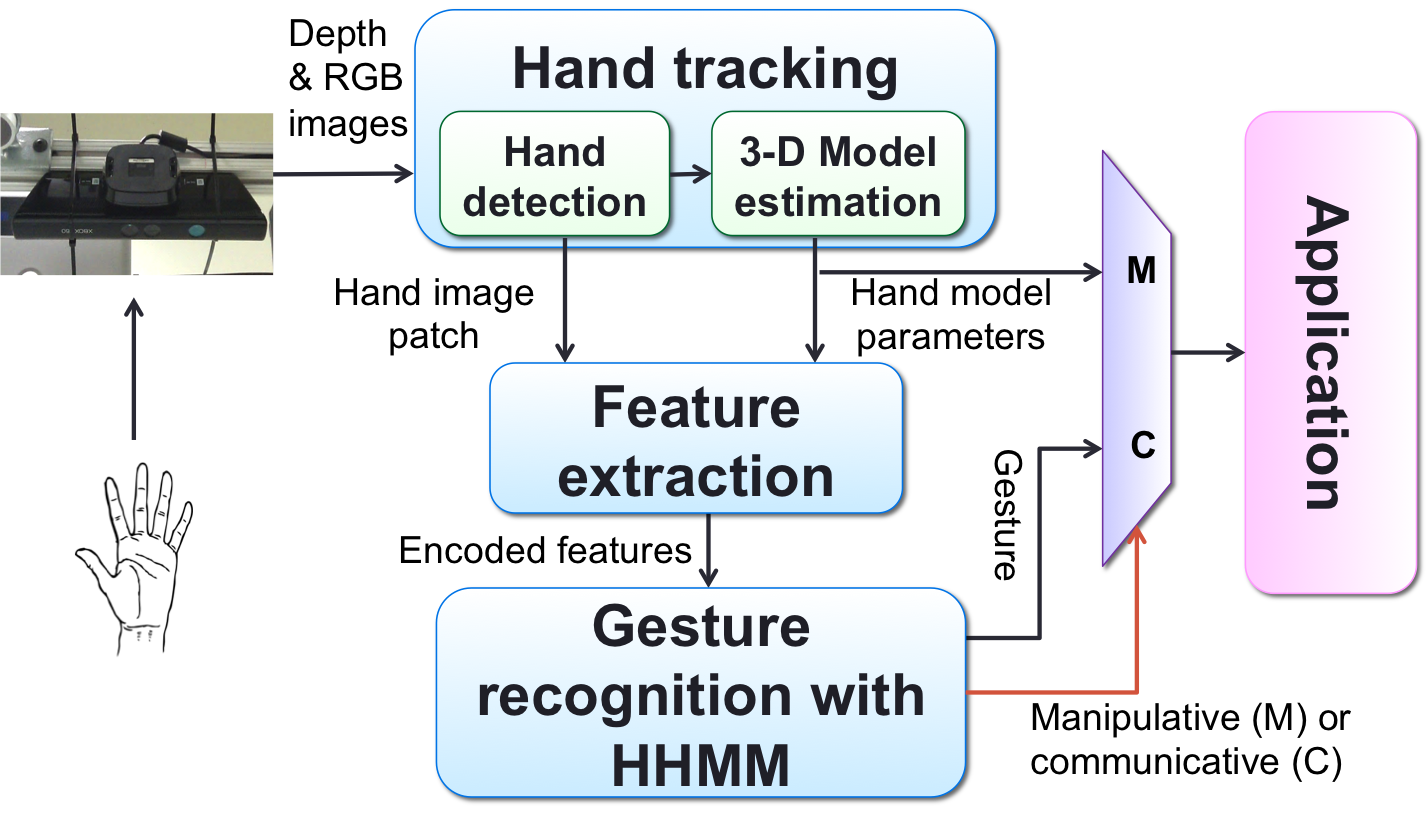
\includegraphics[width=\linewidth]{figures/system_overview.png}
\caption{System overview.}
\label{fig:overview}
\end{figure}

\begin{itemize}
  \item \textbf{Improved hand tracking methods based on gesture salience.}
  I define gesture salience to be proportional to the amount of motion and the
  closeness of the motion to the observer. Based on this, I compute a
  probability map for the gesturing hand locations in a frame. This method
  gives better result than the current Kinect SDK when the hands are closer to
  the body or are moving fast.

  \item \textbf{Fine-grained hand feature extraction.} To handle manipulative
  gestures, I developed algorithms to estimate a simplified 3-D
  skeletal hand model with fingertip positions. For communicative gestures, I am
  comparing different feature descriptors (e.g., histogram of oriented
  gradients) and feature encoding schemes (e.g., principal component analysis,
  sparse coding) for incorporating hand poses into the recognition framework.

  \item \textbf{A unified probabilistic model for gesture recognition.} I am
  developing a framework based on hierarchical hidden Markov
  models (HHMMs) that distinguishes non-gestures, 
  manipulative gestures and communicative gestures in realtime. I am also experimenting with different
  training methods, such as discriminative training and hidden conditional
  random fields, to improve the recognition accuracy. 

  \item \textbf{Online gesture spotting.} A real-time gesture-driven HCI
  application requires gesture spotting with minimum delay. I developed a new
  method for determining the start and the end of a gesture nucleus in
  real-time, while filtering out unintentional hand movement based on
  information from hidden states.
  
  \item \textbf{User interaction techniques.} I identified the importance of
  having both discrete and continuous gestures in a natural interface and how to
  combine them in an interaction interface. I also explored different ways of
  combining gesture and speech for natural interaction.
\end{itemize}

% \subsection{Discriminative Training}
% HMMs as a generative model allows us to model the joint
% distribution of the observed sequence. Traditionally,
% maximum-likelihood (ML) estimation is used to learn the parameters of HMMs. However, our real task is to
% classify the sequence of the observed data. Discriminative classifiers model the
% posterior $p(y|x)$ directly, and hence are believed to give a lower error rate.
% In the speech recognition community, discriminative training methods have been
% proposed and have shown significant improvements over ML-trained models on many
% large vocabulary speech recognition tasks \cite {chang12}. To further improve
% the discriminative power of our model, we will use discriminative training
% methods for gestural analysis.
% 
% HMM provides a computationally efficient modeling framework. The HMM makes two
% main assumptions:
% 
% 1. There exists a hidden state sequence, $S$, that forms a Markov chain that
% generates the observation vectors.
% 
% 2. Given the state $s_t$ at any time point, the corresponding observation $x_t$
% is conditionally independent of other observations and states.
% 
% Instead of seeking model parameters that can maximize the likelihood of the
% data, discriminative training methods seek parameters that can minimize the
% confusions that occur in the training data. In general, discriminative training
% methods consist of two steps: First, construct a smooth and efficient computable
% objective function that reflects the degree of confusion; second, adjust the
% model parameters such that the objective function can be optimized. 
% 
% We will explore several commonly used discriminative training criteria such as
% minimum classification error training, maximum mutual
% information training, and margin-based training methods. For optimizing
% parameters, we can use either the extended Baum-Welch method or gradient-based
% methods. We will also compare the results to those without discriminative
% training and those with CRF-based models.

% \subsection{Motivating Application}
% We will develop a simple game-like application that simulates some of the USAR
% interaction scenarios. The game will be browser-based for easy access. With the
% recent development in HTML5, browser-based interaction becomes richer and
% richer. Web browsers have become the main application people use to do various
% tasks because they provide better accessibility to information via the
% Internet. We believe that being able to use gesture as an input to the browser
% will make a big contribution to HCI as well.
% 
% The game we have in mind is highly inspired by
% StarCraft\footnote{http://us.battle.net/sc2/en/}. StarCraft is a real-time
% strategic game that involves controlling different kinds of units to accomplish
% a vast array of tasks. The game's richness in command and control can help us develop a set of gestural language in this domain.
% 
% The gestural input functionality we want demonstrate in this application are:
% 
% \begin{enumerate}
%   \item Moving units from one location to another
%   \item Panning the map
%   \item Command a unit to build different kinds of buildings, like recycler,
%   barrack, and factory etc.
%   \item Command units to attack the enemies by doing an attack gesture (say
%   ``attack'') and pointing to the location of attack
% \end{enumerate}

% \subsection{User Study}\label{sec:user_study}
% We will bootstrap the system with a set of natural gestures defined based on the
% user studies done by Yin et al. \cite{yin10} and Wobbrock et al.
% \cite{wobbrock09} on the set of natural gestures people do for surface
% computing. We will conduct a user study after making a simple application where
% the user can perform both manipulative and communicative gestures. The goal of 
% the user study is to evaluate the accuracy of the hand tracking and gesture 
% recognition. A research question here is whether we can bootstrap the system 
% only with the gesture examples we provide ourselves, or we need to collect 
% training examples from the users, and how well the system performs 
% independent of users.

% \section{Appendix A - Review of Kalman Filter}
% Let $x_k$ be an $n$-dimensional vector of state components and $P_k$ be the
% $n$-by-$n$ error covariance. The measurement $z_k$ is an $m$-dimensional
% vector given by:
% \begin{align*}
% z_k = H_kx_k + v_k,
% \end{align*}
% where $H_k$ is an $m$-by-$n$ matrix and $v_k$ is the measurement error.
% 
% The \textit{Kalman gain}, $K_k$, is an $n$-by-$m$ matrix expressed as:
% \begin{align*}
% K_k = P_k^-H_k^T(H_kP_k^-H_k^T + R_k)^{-1}
% \end{align*}
% 
% Assuming no external control, the a priori estimate $x_k^-$ of the state is
% given by:
% \begin{align*}
% x_k^- = Fx_{k - 1} + w_k,
% \end{align*}
% where $F$ is the $n$-by-$n$ \textit{transfer matrix} characterizing the
% dynamics of the system, and $w_k$ is the \textit{process noise} associated with
% random events or forces that directly affect the actual state of the system. We assume that the components of $w_k$
% have Gaussian distribution $N(0, Q_k)$ for some $n$-by-$n$ covariance matrix
% $Q_k$.
% 
% Using $P_k^-$ to denote the error covariance, the a priori estimate for this
% covariance at time $k$ is obtained from the value at time $k - 1$ by:
% \begin{align*}
% P_k^- = FP_{k - 1}F^T + Q_{k - 1}
% \end{align*}
% 
% The updated value for $x_k$ when a new measurement is available is:
% \begin{align*}
% x_k = x_k^- + K_k(z_k^- - H_kx_k^-)
% \end{align*}
% The update value for $P_k$ is:
% \begin{align*}
% P_k = (I - K_kH_k)P_k^-
% \end{align*}
% 

% 
% \section{Appendix C - Review of Random Conditional Fields}
% Each clique template $C_p$ is a set of factors which has a corresponding set
% of sufficient statistics $\{f_{pk}(\mathbf{x_p}, \mathbf{y}_p)\}$ and
% parameters $\theta_p\in\mathcal{R}^{K(p)}$. The CRF can be written as
% \begin{align}
% p(\mathbf{y}|\mathbf{x}) = \frac{1}{Z(\mathbf{x})}\prod_{C_p\in
% \mathcal{C}}\prod_{\Psi_c\in C_p}\Psi_c(\mathbf{x}_c,
% \mathbf{y}_c;\theta_p)
% \end{align}
% where each factor is parameterized as
% \begin{align}
% \Psi_c(\mathbf{x}_c, \mathbf{y}_c;\theta_p) =
% \exp\left\{\sum_{k=1}^{K(p)}\lambda_{pk}f_{pk}(\mathbf{x}_c,
% \mathbf{y}_c)\right\}
% \end{align}
% and the normalization function is 
% \begin{align}
% Z(\mathbf{x}) 
% &= \sum_{\mathbf{y}}\prod_{C_p\in\mathcal{C}}\prod_{\Psi_c\in
% C_p}\Psi_c(\mathbf{x_c}, \mathbf{y_c}; \theta_p)\\
% &= \sum_{\mathbf{y}}\exp\left\{\sum_{C_p\in\mathcal{C}}\sum_{\Psi_c\in
% C_p}\sum_{k=1}^{K(p)}\lambda_{pk}f_{pk}(\mathbf{x}_c,
% \mathbf{y}_c)\right\}
% \end{align}
% 
% The conditional log likelihood is given by 
% \begin{align}
% \ell(\theta) = \sum_{C_p\in\mathcal{C}}\sum_{\Psi_c\in
% C_p}\sum_{k=1}^{K(p)}\lambda_{pk}f_{pk}(\mathbf{x}_c, \mathbf{y}_c) - \log Z(\mathbf{x})
% \end{align}
% 
% The partial derivative of the log likelihood with respect to a parameter
% $\lambda_{pk}$ associated with a clique template $C_p$ is
% \begin{align}
% \frac{\partial\ell}{\partial\lambda_{pk}} 
% &= \sum_{\Psi_c\in C_p}\lambda_{pk}f_{pk}(\mathbf{x}_c, \mathbf{y}_c) -
% \frac{1}{Z(\mathbf{x})}\frac{\partial Z(\mathbf{x})}{\partial\lambda_{pk}}\\
% &= \sum_{\Psi_c\in C_p}\lambda_{pk}f_{pk}(\mathbf{x}_c, \mathbf{y}_c) -
% \frac{1}{Z(\mathbf{x})}\sum_{\mathbf{y}}\exp\left\{\sum_{C_p\in\mathcal{C}}\sum_{\Psi_c\in
% C_p}\sum_{k=1}^{K(p)}\lambda_{pk}f_{pk}(\mathbf{x}_c,
% \mathbf{y}_c)\right\}\sum_{\Psi_c\in C_p}f_{pk}(\mathbf{x}_c, \mathbf{y}_c) \\
% &= \sum_{\Psi_c\in C_p}\lambda_{pk}f_{pk}(\mathbf{x}_c, \mathbf{y}_c) -
% \frac{1}{Z(\mathbf{x})}\sum_{\mathbf{y}}p(\mathbf{y}, \mathbf{x})\sum_{\Psi_c\in
% C_p}f_{pk}(\mathbf{x}_c, \mathbf{y}_c) \\
% &= \sum_{\Psi_c\in C_p}\lambda_{pk}f_{pk}(\mathbf{x}_c, \mathbf{y}_c) -
% \frac{1}{Z(\mathbf{x})}\sum_{\Psi_c\in C_p}\sum_{\mathbf{y}}p(\mathbf{y},
% \mathbf{x})f_{pk}(\mathbf{x}_c, \mathbf{y}_c) \\
% &= \sum_{\Psi_c\in C_p}\lambda_{pk}f_{pk}(\mathbf{x}_c, \mathbf{y}_c) -
% \frac{1}{Z(\mathbf{x})}\sum_{\Psi_c\in C_p}\sum_{\mathbf{y'_c}}p(\mathbf{y'_c},
% \mathbf{x})f_{pk}(\mathbf{x}_c, \mathbf{y'}_c) \\
% &= \sum_{\Psi_c\in C_p}\lambda_{pk}f_{pk}(\mathbf{x}_c, \mathbf{y}_c) -
% \sum_{\Psi_c\in C_p}\sum_{\mathbf{y'_c}}f_{pk}(\mathbf{x}_c, \mathbf{y}_c)p(\mathbf{y'_c}
% | \mathbf{x})
% \end{align}